\documentclass{article}
\usepackage[utf8]{inputenc}
\usepackage[a4paper, total={6in, 8in}]{geometry}
\usepackage{graphicx}
\usepackage{amsmath}
\usepackage{amssymb}
\usepackage{booktabs} % for "\midrule" macro
\usepackage{lipsum} % for filler text
\usepackage{enumerate}
\usepackage{amsmath}
\usepackage{array}
\usepackage{lplfitch}
\usepackage{hyperref}
\usepackage{caption}

\newcommand*\moveToRight[1]{\hspace*{0em plus 1fill}\makebox{(#1)}}
\newcommand*\fixindent{ \hspace{1pt}\\}
%this command below is not my work was used for quality of life
%link to original post 
%https://tex.stackexchange.com/questions/330588/how-to-produce-given-number-of-quad-in-math
\newcommand{\myquad}[1][1]{\hspace*{#1em}\ignorespaces}
\title{Assignment Two}
\author{Abanob Tawfik\\z5075490}
\date{March 2019}

\begin{document}
\maketitle
\section{Problem 1}
Use Natural Deduction to show the following: \moveToRight{10 marks}\\
\begin{center}
$\vdash P(a)\to \forall x(P(x) \lor \neg(x = a))$    
\end{center}

        Solution:\\
        \fitchprf{}{
            \subproof{\pline[1.]{$\neg (P(a)\to \forall x(P(x) \lor \neg(x = a))$}}{
                \subproof{\pline[2.]{$P(a)$}}{
                    \subproof{\pline[3.]{$\neg(P(b) \lor \neg (b = a))$}}{
                        \subproof{\pline[4.]{$\neg P(b)$}}{
                            \subproof{\pline[5.]{$b = a$}}{
                                \pline[6.]{$\neg P(a)$} \eqe{4}{5}\\
                                \pline[7.]{$\bot$} \lfalsei{2}{6}
                            }
                            \pline[8.]{$\neg(b = a)$} \lnoti{5--7}\\
                            \pline[9.]{$P(b) \lor  \neg(b = a)$}[$\lor$ Intro-2: 8]\\
                            \pline[10.]{$\bot$}\lfalsei{3}{9}
                        }
                        \pline[11.]{$\neg\neg P(b)$} \lnoti{4--10}\\
                        \pline[12.]{$P(b)$}[Double Negation Elim: 11]\\
                        \pline[13.]{$P(b) \lor \neg(b = a)$}[$\lor$ Intro-1: 12]\\
                        \pline[14.]{$\bot$}\lfalsei{3}{13}
                    }
                    \pline[15.]{$\neg\neg(P(b) \lor \neg(b = a))$} \lnoti{3--14}\\
                    \pline[16.]{$(P(b) \lor \neg(b = a))$}[Double Negation Elim: 15]\\
                    \pline[17.]{$\forall x(P(x) \lor \neg(x = a))$} \lalli{16}
                }
                \pline[18.]{$P(a) \to\forall x(P(x) \lor \neg(x = a))$} \lifi{2--17}\\
                \pline[19.]{$\bot$}\lfalsei{1}{18}
            }
            \pline[20.]{$P(a) \to\forall x(P(x) \lor \neg(x = a))$} [IP: 1-19]
        }\\\\
        Since i had used a derived rule "Double Negation Elim" i will also provide a proof for this rule on the next page. 
        
\newpage
\fixindent{}
Proof for "Double Negation Elim"\\
\begin{center}
$\neg\neg \psi(a)\vdash \psi(a))$    
\end{center}
Solution:\\
 \fitchprf{\pline[1.]{$\neg\neg \psi(a)$}}{
            \subproof{\pline[2.]{$\neg \psi(a)$}}{
                \pline[3.]{$\bot$}\lfalsei{1}{2}
            }
            \pline[4.]{\psi(a)}[IP: 1-3]
        }\\\\
Explanation of the proof:\\
\fixindent{}
This proof has no premises, so in order to perform a proof of such we need an indirect proof which can also be seen as proof by contradiction. First we assume the opposite of what we are trying to prove, in this case the negation of our consequence:
\fixindent{}
\hspace*{150pt}$\neg(P(a) \to \forall x(P(x) \lor \neg(x = a)))$\\\fixindent{}
Next we want to try to arrive to the contradiction somewhere down the proof. We use modus ponen by assuming $P(a)$ and trying to reach the conclusion in the subproof $\forall x(P(x) \lor \neg(x = a))$ allowing us to introduce implication and arrive to a direct contradiction:
\fixindent{}
\hspace*{150pt}$P(a) \to \forall x(P(x) \lor \neg(x = a))$
\fixindent{}\fixindent{}
We want to make the assumption of the negation of the conclusion we are trying to reach using variable b, as when b is no longer a free variable in x, in other words we are no longer working under the assumption $P(b)$ and b is arbitrary we can perform a $\forall$ introduction.\\
\fixindent{}
Since the consequence $\forall x(P(x) \lor \neg(x = a))$ contains $\lor$, we only need one side of the predicate to perform a $\lor$ introduction. To do this properly and allow use of the $\forall$ introduction we need to make b an arbitrary variable. We make the assumption $\neg P(b)$ and under that we make another assumption b = a. By doing this we can perform an equals elimination (substitution) to arrive at $\neg P(a)$ which is a direct contradiction to our first assumption $P(a)$. This gives us $\bot$ which implies $\neg (b = a)$ and this can also be done to imply $P(b)$ similarly.\\
\fixindent{}
By having the above under the assumption $\neg(P(b) \lor \neg(b = a))$ we can perform a $\lor$ introduction on $P(b)$ above to introduce $\neg(b = a)$ arriving at P(b) $\lor$ $\neg(b = a)$ which is again another contradiction. Since this subproof concludes to $\bot$ we can assume the negation of our initial assumption for the subproof which is $P(b) \lor \neg(b = a)$. Because b is an arbitrary variable, $\neg P(b)$ was discharged, we can simply perform a $\forall$ introduction and arrive to the conclusion:\\
\hspace*{150pt}$P(a) \to \forall x(P(x) \lor \neg(x = a))$
\fixindent{}
\fixindent{}
This is a direct contradiction to our initial assumption $\neg(P(a) \to \forall x(P(x) \lor \neg(x = a)))$, giving us $\neg\neg(P(a) \to \forall x(P(x) \lor \neg(x = a)))$. Performing one more double negation elimination (proven in the second natural deduction proof) gives us the following conclusion by indirect proof:
\fixindent{}
\fixindent{}
\hspace*{150pt}$\vdash P(a)\to \forall x(P(x) \lor \neg(x = a))$
\newpage
\begin{flushleft}
The following images below were taken from the following natural deduction verification tool,  \href{https://proofs.openlogicproject.org/}{https://proofs.openlogicproject.org/}, which was used to validate the following natural deduction that was performed in the problem and the proof of the derived rule for double negation elimination. Note that rule DNE was used  on the image, this was a derived rule that was proven and verified in the next image.\\
\end{flushleft}
\begin{centering}\hspace*{1pt}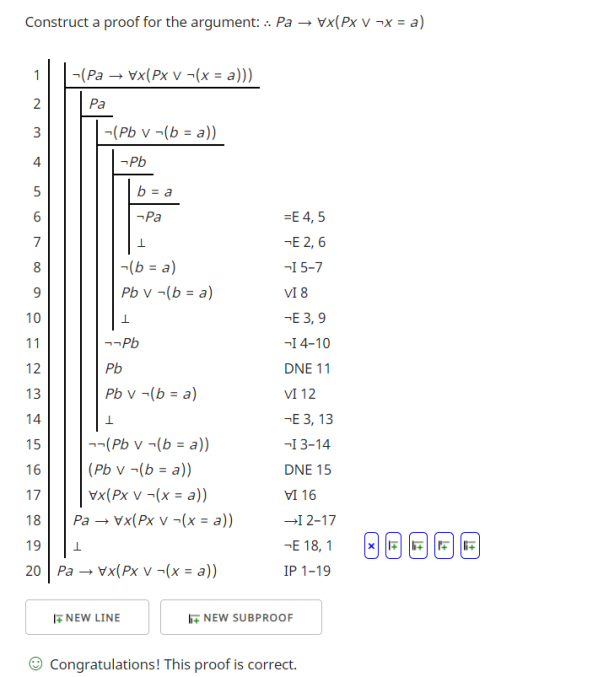
\includegraphics[width=400px, height = 400px]{p2.png}\captionof{figure}{Verification tool returning that my proof is correct for main proof}\end{centering}
\newpage
\begin{flushleft}
Below is the image showing the proof for the derived rule DNE which states that $\neg\neg P = P$.\\
\begin{centering}\hspace*{1pt}\\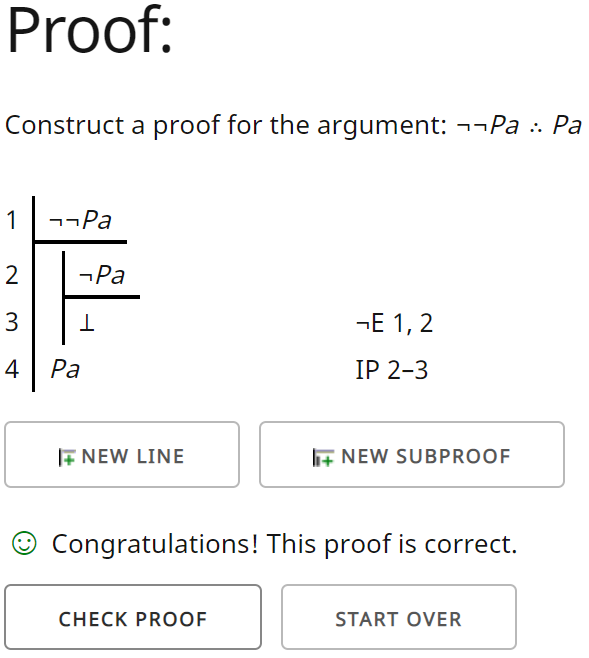
\includegraphics[width=300px, height = 300px]{p1.png}\captionof{figure}{Verification tool returning that my proof of the derived rule DNE is correct}\end{centering}
\end{flushleft}
\newpage
\section{Problem 2}

\end{document}
